This section is the \textbf{logical/functional view} of the Y layer (conforming to the Logical/Functional viewpoint declared in Section 3). The layer is decomposed into its subsystems, and the responsibilities, interfaces, and data flows of each subsystem are defined. A subsystem is a programming unit that implements one of the major functions of the layer and serves as a source/sink of data for other subsystems. Describe each subsystem in a separate subsection using the same structure. Include any special considerations or trade-offs for the approach chosen.

\subsection{Subsystem 1}
A general description of this subsystem. For most subsystems, an extract of the architectural block diagram with data flows is useful --- showing this subsystem and those it communicates with.

\begin{figure}[h!]
	\centering
 	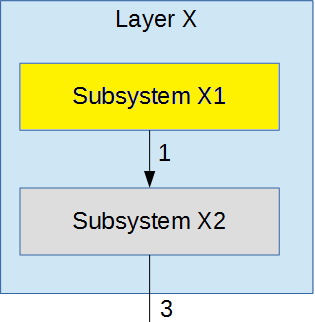
\includegraphics[width=0.60\textwidth]{images/subsystem}
 \caption{Example subsystem description diagram}
\end{figure}

\subsubsection{Assumptions}
Any assumptions made in defining the subsystem. Pay particular attention to assumptions concerning interfaces and interactions with other layers.

\subsubsection{Responsibilities}
Expand each responsibility/feature/function/service of this subsystem, as identified in the architectural overview, into more detailed responsibilities. Clearly describe what the subsystem does (and does not do).

\subsubsection{Subsystem Interfaces}
Define each input and output for the subsystem. Create one row per labelled interface that connects to this subsystem, describing the incoming and outgoing data elements. Interface identifiers use the scheme declared in Section 3 and are the anchors for requirements traceability.

\begin {table}[H]
\caption {Subsystem interfaces}
\begin{center}
    \begin{tabular}{ | p{1cm} | p{6cm} | p{3cm} | p{3cm} |}
    \hline
    ID & Description & Inputs & Outputs \\ \hline
    \#01 & Description of the interface/bus & \pbox{3cm}{input 1 \\ input 2} & \pbox{3cm}{output 1}  \\ \hline
    \#02 & Description of the interface/bus & \pbox{3cm}{N/A} & \pbox{3cm}{output 1}  \\ \hline
    \end{tabular}
\end{center}
\end{table}

\subsubsection{Design Rationale}
Briefly justify this subsystem's boundary and approach: why these responsibilities are grouped together, and any significant alternatives considered. Record architecturally significant choices as decisions in Section 9 and reference them here (e.g. ``per AD-02'').

\subsection{Subsystem 2}
Repeat for each subsystem.

\subsection{Subsystem 3}
Repeat for each subsystem.
